\section{Modularity}
\label{sec:modularity}

Since the framework developed in the course of this thesis is required to be highly modular, we first need to define the term \textit{Modularity}, find out how it relates to software engineering and choose a tool for supporting modularity on the Java platform.

Modularity is a frequently used term in Software Engineering. To understand the fundamental concept of it, take a look at the following definitions:

\begin{quote}
Large software systems are inherently more complex to develop and maintain than smaller systems. Modularity involves breaking a large system into separate physical entities that ultimately makes the system easier to understand.

\hfill \textbf{Java Application Architecture}

\hfill \citeauthor{Knoernschild:2012} \cite{Knoernschild:2012}
\end{quote}

\begin{quote}
Systems are deemed “modular” when they can be decomposed into a number of components. The components are able to connect, interact, or exchange resources in some way, by adhering to a standardized interface. Unlike a tightly integrated product whereby each component is designed to work specifically with other particular components in a tightly coupled system, modular products are systems of components that are loosely coupled.

\hfill \textbf{Modularity}

\hfill \citeauthor{Wikipedia:Modularity:2012} \cite{Wikipedia:Modularity:2012}
\end{quote}

Basically, modularity is based on modules, their requirements and behaviour. To fully understand the meaning of modularity we need to focus on the \textit{module} itself:

\subsection{Module definition}
\label{sec:module}

According to \citeauthor{Knoernschild:2012}, a software module is defined as follows:

\begin{quote}
A software module is a deployable, manageable, natively reusable, composable, stateless unit of software that provides a concise interface to consumers. 

\hfill \textbf{Java Application Architecture}

\hfill \citeauthor{Knoernschild:2012} \cite{Knoernschild:2012}
\end{quote}

Figure \ref{fig:module} illustrates this defnition and all the individual aspects of a module \cite{Knoernschild:2012}.

\begin{figure}[H]
\centering
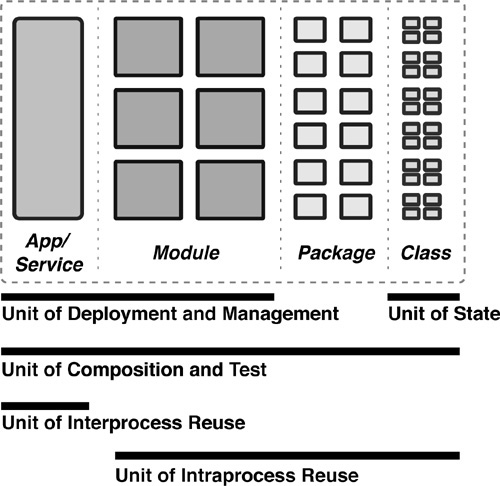
\includegraphics[width=0.8\textwidth]{module.jpeg}
\caption{Module definition diagram}
\label{fig:module}
\end{figure}

\subsection{OSGi}
\gls{OSGi} is the most widely used and highly developed module system and service platform for the Java environment. This chapter aims to show why \gls{OSGi} is the best choice for building highly modular Java-based software systems as it supports all requirements of modularity defined by \citeauthor{Knoernschild:2012} \cite{Knoernschild:2012}.

The \gls{OSGi} technology is a set of specifications that define a dynamic component system for Java. These specifications enable a development model where applications are dynamically composed of many different reusable components. The \gls{OSGi} specifications enable modules to hide their implementations from other modules while communicating through services, which are objects that are specifically shared between modules. This surprisingly simple model has far reaching effects for almost any aspect of the software development process \cite{OSGi}. In \gls{OSGi} parlance, a module is known as a bundle. \gls{OSGi} provides a framework for managing bundles that are packaged as regular Java JAR files with an accompanying manifest. The manifest contains important metadata that describes the bundles and its dependencies to the \gls{OSGi} framework \cite{Knoernschild:2012}. Figure \ref{fig:layering-osgi} shows the layered model architecture of the \gls{OSGi} service platform.

\begin{figure}[H]
\centering
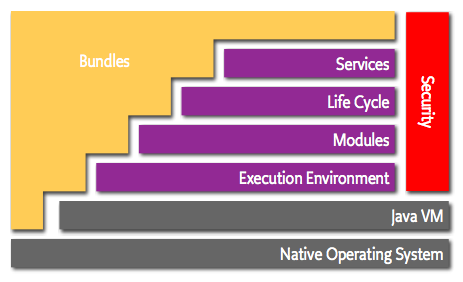
\includegraphics[width=0.73\textwidth]{layering-osgi.png}
\caption{\gls{OSGi} layered model \cite{OSGi}}
\label{fig:layering-osgi}
\end{figure}

\subsubsection{Implementations}
\gls{OSGi} is the foundation for many different Application Servers and IDEs. Some of the most widely used open source implementations of the \gls{OSGi} specification are listed here: 

\begin{itemize}
	\item \textbf{Eclipse Equinox} \\
		\url{http://eclipse.org/equinox/} \\
		Equinox is the core of the plug-in runtime for the Eclipse IDE.
	\item \textbf{Apache Felix} \\
		\url{http://felix.apache.org/} \\
		Apache Felix is the open source \gls{OSGi} implementation powered by the \gls{ASF} and is the basis of several other Apache projects like Apache Aries and Apache Karaf.
	\item \textbf{Knopflerfish} \\
		\url{http://www.knopflerfish.org/} \\
		Knopflerfish is the spin-off from one of the \gls{OSGi} alliance founding members and was open-sourced in 2003.
\end{itemize}

The developed framework uses Apache Felix for bundle testing purposes but aims to be \gls{OSGi} compliant and implementation independence. Apache Felix was chosen for its easy configuration and small memory footprint.

\gls{OSGi} is considered to be the most advanced module system for the Java platform. It supports all aspects of modularity, such as deployability, manageability, reusability and composability. Since modularity and its benefits and advantages, such as maintainability, is one of the main requirement of this work, \gls{OSGi} is the best choice as a foundation for the framework. 

\subsection{Relevant principles and design patterns}
\label{sec:patterns}
Some of the most important aspects of modular software design, in the form of principles and design patterns, will be discussed on the following pages. The findings derived from these patterns influenced the way the framework was designed and implemented, as shown in chapter \ref{sec:design} (pp. \pageref{sec:design}ff).

\subsubsection{Single Responsibility Principle}
The term \textit{Single Responsibility Principle} was first introduced by Robert C. Martin in his book \citetitle{Martin:2002} \cite{Martin:2002}. It states that every class should have one, and only one, responsibility. The principle is originally coined for \gls{OOD} but can easily be adapted to module design. The reason for keeping a class or module focused on a single concern is that it makes the class or module more robust, since changing a class increases the danger of other parts of it to break. Applied to concrete module design one could say that if a module is concerned with two aspects of a problem it should be separated into two different modules. 

\subsubsection{Dependency Inversion Principle}
The \textit{Dependency Inversion Principle} again was postulated by Robert C. Martin and states that High-level modules should not depend on low-level modules. Both should depend on abstractions \cite{Martin:2002}. The problem with the traditional approach, higher-level components depending on lower-level components, limits the higher-level components reusability because the modules are too tightly coupled. The dependency inversion principle allows to increase the reusability of higher-level modules by allowing to choose from different lower-level implementations. In the context of module design it's important to depend on modules with a well-defined interface. The best way to enforce the replaceability of lower-level modules is to introduce interface modules which solely contain the \gls{API} for a component. Implementors of this interface can then be swapped during runtime. In concrete systems this usually results in \gls{API} and implementation modules. Modules should then only depend on \gls{API} modules but never on implementation modules.

\subsubsection{Dependency Injection}
\gls{DI} is way too solve the problem described by the \textit{Dependency Inversion Principle}.
\gls{DI} is an expression introduced by Martin Fowler in its article \textit{Inversion of Control Containers and the Dependency Injection Pattern} \cite{Fowler:2004}. Dependency Injection specifies the means for obtaining objects in such a way as to maximize reusability, testability and maintainability compared to traditional approaches such as constructors, factories, and service locators \cite{JSR330}. \gls{DI} does this by allowing a class to specify its dependencies and rely on their provision at runtime rather than retrieving them explicitly. This leaves the programmer's code clean, flexible, and relatively free of dependency-related infrastructure \cite{JSR330}.

The main reason why \gls{DI} works well with modularity is the fact, that it main purpose is dependency management which is also very important when designing and implementing modular systems. \gls{DI} forces clients to be honest about their dependencies instead of hiding them in implementation details, which allows clients using modules to quickly get a realistic view of what the module is supposed to do and what dependencies it requires to do so.

\subsection{Supporting libraries and tools}
There are several freely available Java libraries and build tools that solve some of the problems when designing modular software in general and for the \gls{OSGi} platform in particular. All of the libraries and tools described in this chapter will be used in the design and implementation of the framework.

\subsubsection{Guice}
Guice is a lightweight dependency injection framework for Java \cite{Guice}. It's Open Source and available on \url{https://code.google.com/p/google-guice/}.

The typical code to implement Guice is shown in the following two listings. The first shows a simple \textit{Module}. Modules in Guice are usually used to bind interfaces to concrete classes.

\begin{listing}[H]
\begin{minted}{java}
public final class ProcessModule extends AbstractModule {

    @Override 
    protected void configure() {
        bind(ProcessService.class).to(DefaultProcessService.class);
    }

}
\end{minted}
\caption{Guice module}
\end{listing}

In your classes you usually define a single constructor, annotated with \texttt{@Inject}, and all required dependencies as parameters. The construction of instances and the dependency resolution is done by Guice, no additional boilerplate code is necessary.

\begin{listing}[H]
\begin{minted}{java}
final class DefaultEngine implements Engine {

    private final ProcessService service;

    @Inject
    DefaultEngine(ProcessService service) {
        this.service = service;
    }

}
\end{minted}
\caption{Constructor injection}
\end{listing}

\subsubsection{Guice Extensions}
Guice has an extensible plug-in mechanism which allows third parties to provide additional functionality. Banshie uses two official Guice extension extensively: Assisted Inject\footnote{\url{https://code.google.com/p/google-guice/wiki/AssistedInject}} and Multibindings\footnote{\url{https://code.google.com/p/google-guice/wiki/Multibinding}}. Assisted Inject allows the combination of Guice-provided dependencies and user-provided parameters on a single injection point. Multibindings supports the binding and injection of Sets and Maps.

\paragraph{Peaberry}
Guice has no native OSGi support, apart from maybe the OSGi-compatible bundle manifest. To overcome this shortcoming, Peaberry\footnote{\url{https://code.google.com/p/peaberry/}}, a third-party open-source Guice extension, offers OSGi-Guice bridge capabilities. It offers \gls{DI} of OSGi dynamic services via Guice's common injection mechanisms and provides a rich and typesafe API to deal with the OSGi service registry and lifecycle events. Listing \ref{lst:peaberry-lifecycle} shows the usage of Peaberry's lifecycle annotations.

\begin{listing}[H]
\begin{minted}{java}
import org.ops4j.peaberry.activation.Start;

public class DefaultCorpusRepository implements CorpusRepository {

    private File basePath = new File("corpora");

    @Start
    public void onStart() {
        basePath.mkdirs();
    }

}
\end{minted}
\caption{Peaberry lifecycle annotation}
\label{lst:peaberry-lifecycle}
\end{listing}

Peaberry even supports the automatic \gls{DI} context creation upon bundle start by using an OSGi extender bundle. Bundles just need to provide the following bundle header to trigger an execution:

\begin{listing}[H]
\texttt{Bundle-Module: org.whiskeysierra.banshie.execution.ExecutionModule}
\caption{Peaberry bundle header}
\end{listing}

Peaberry creates one \texttt{Injector} per bundle, any interaction between bundles is based on standard OSGi services, which allows to combine Peaberry-aware bundles and normal ones.

\subsubsection{BND Tool and the Maven Bundle Plugin}
With \gls{OSGi} you are forced to provide additional metadata in the JAR's manifest to verify the consistency of your classpath. This metadata must be closely aligned with the class files in the bundle. Maintaining this metdata is an error prone chore because many aspects are redundant. The core task of the BND Tool is to analyze the class files and find every dependency. These dependencies are then merged with instructions supplied by the user \cite{BND}. Since Banshie uses Apache Maven for building its independent modules, the natural choice was to use a Maven Plugin for this, which is provided by the Apache Felix Maven Bundle Plugin \footnote{\url{http://felix.apache.org/site/apache-felix-maven-bundle-plugin-bnd.html}}. The following listing shows the bare minimum of configuration code to use the Maven Bundle Plugin in a POM file.

\begin{listing}[H]
\begin{minted}{xml}
<packaging>bundle</packaging>
...
<build>
    <plugins>
        <plugin>
            <groupId>org.apache.felix</groupId>
            <artifactId>maven-bundle-plugin</artifactId>
        </plugin>
    </plugins>
</build>
\end{minted}
\caption{Maven Bundle Plugin usage}
\end{listing}

\subsection{Summary}
This chapter focused on the modularity aspect of this thesis. We discussed the concept of modularity, how it relates to module design and why \gls{OSGi} is the best available module system for the Java platform at the moment. Additionally some relevant patterns, principles and libraries, which are closely related to modular software design and implementation, were described and discussed. 